% !TEX root = ../../thesis.tex
%______________________________________________________________________________
%
% SECTION
\section{The Spectral Element Method}
\label{section:sem}
%
%______________________________________________________________________________

As pointed out in section \ref{section:wave_equation}, a diagonal mass matrix $\mathbf M$ is essential to fully exploit the efficiency of explicit time integration schemes. A well-established approach that yields an inherently diagonal consistent mass matrix, is the Spectral Element Method (SEM) \cite{Maggio1994}. Based on the p-version of the FEM, the SEM relies on a specific choice of ansatz space and quadrature rule for its appealing properties.

Using the same line of thought as for the simplification of the moment fitting equations described in section \ref{section:fcm}, Lagrange polynomials defined on a set of Gauss-Lobatto points are used as basis functions. Accordingly, the quadrature rule for integrating the mass matrix is the Gauss-Lobatto scheme of matching order, which means that the integration points coincide with those used for the definition of the basis functions. As a result, the product of mixed ansatz functions vanish at all integration points, leading to a diagonal mass matrix.

\begin{equation}
	N_i(\boldsymbol{\xi}_k)N_j(\boldsymbol{\xi}_k) = 0 \ \ \forall i \neq j \ \ \forall k \in \{1..m\}
\end{equation}

\begin{equation}
	M_{ij} = \int_{\Omega} N_i \rho N_j d\mathbf x
	\approx
	det(\mathbf J) \sum_{k=1}^m N_i(\boldsymbol{\xi}_k) \rho N_j(\boldsymbol{\xi}_k) w_k
	=
	\begin{bmatrix}
		M_{11} & & \\
		& \ddots & \\
		& & M_{nn} \\
	\end{bmatrix}
\end{equation}

where $\mathbf J$ is the Jacobian facilitating the change of variables from $\mathbf x$ to $\boldsymbol{\xi}$.

Gauss-Lobatto points are chosen in particular because they always include the limits of the integration domain $-1$ and $1$, ensuring that all except one ansatz functions vanish on each border, as shown in figure \ref{fig:lagrange_basis}. This property is essential for FE-based methods to ensure the continuity between elements, allow the blending of specific ansatz functions to exactly capture certain types of boundaries, and strongly enforce boundary conditions.

\begin{figure}[h]
	\centering
	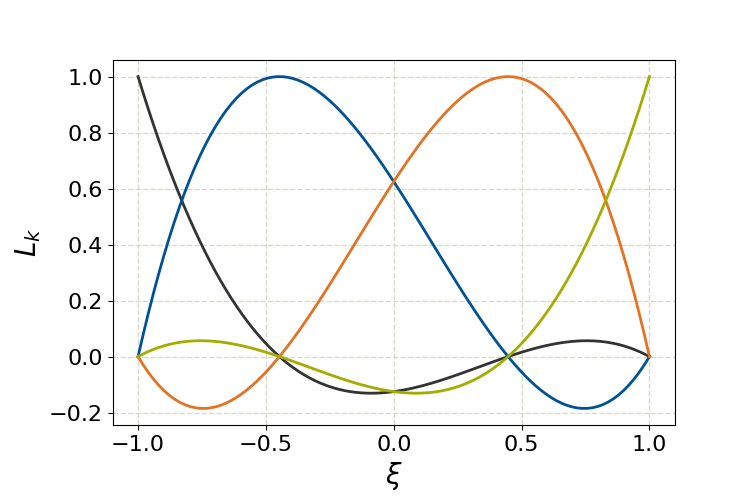
\includegraphics[height=6cm]{pictures/figures/lagrange_basis.png}
	\caption{Lagrange basis functions on a set of fourth order Gauss-Lobatto points.}
	\label{fig:lagrange_basis}
\end{figure}

Using a Lagrange basis instead of integrated Legendre polynomials has some unpleasant consequences. Firstly, the hierarchic nature of the ansatz space is lost, requiring the entire re-evaluation of all structural matrices when performing p-refinement. Moreover, the conditioning of the stiffness matrix is no longer optimal \cite{Zumbusch1996} but degrades with increasing $p$. Lastly, no complete trunk space of Lagrange polynomials exist, which means that the ansatz space must be constructed from the tensor product of the basis functions, leading to an increased number of degrees of freedom and requiring more computational resources.
On the other hand, Lagrange basis functions are nodal and have a partition of unity $\sum_{k=1}^m L_k(\xi) = 1$, which makes lumping procedures possible and simple.

To ensure the diagonality of the mass matrix, the basis functions' polynomial order $p$ uniquely defines the quadrature scheme as the tensor product of $m=p+1$ order Gauss-Lobatto rule, leading to further undesirable effects. The most obvious one of course is the lack of choice when it comes to the selection integration schemes.
This greatly limits the types of problems the SEM is applicable to, since the set of exactly integrable polynomials becomes limited, restricting the total polynomial order of the integrands in equation \ref{eq:structural_components}. The highest polynomial order a tensor product quadrature scheme is able to exactly integrate is identical to that of the underlying 1D rule for each variable \cite{Keister1996}. In the case of SEM, this translates to $2m-3=2p-1$. Considering \ref{eq:structural_components}, the highest order of the mass matrix's integrand is $2p$ per direction, while the stiffness matrix's is $2p-1$ in 1D and $2p$ in higher dimensions. Consequently, neither the mass nor the stiffness matrix can be integrated exactly (apart from 1D models), even for constant material parameters.

Since the stiffness matrix does not benefit from using the Gauss-Lobatto rule in any way, a different integration scheme can be applied. Unfortunately, no solution exists to this problem in the mass matrix's case, meaning that it is always underintegrated in the SEM. It is important to note that under certain circumstances, especially in wave propagation problems, this drawback partly balances other errors originating from the discretization \cite{Ainsworth2010}, leading to more accurate results when compared to the classical FEM. In general however, it is an additional source of errors and a restriction that limits the physical models to linear ones.

Main ideas to go through:

The primary feature of the SEM is that it provides an inherently diagonal mass matrix that
lends itself well to using explicit finite differences in time. By carefully choosing the
basis functions and the integration scheme, the mass matrix becomes diagonal without any
additional lumping required.

The underlying idea of the SEM is to use a set of Lagrange polynomials as basis functions,
interpolating all integration points.
% TODO: figure showing lagrange polynomials
This means that at each integration point, only one
basis function has a non-zero value, rendering all products of mixed basis functions zero
at that point. Since the product of basis function pairs appears as a coefficient in the
integrand of the mass matrix, all non-diagonal components vanish.

However, a couple of requirements constrain the choice of integration points. First of all,
in every FE-based method, each boundary of an element needs at least one basis function that does not vanish on it.
In the context of SEM, this requirement manifests as having exactly one non-zero basis function per
element boundary with its own set of integration points on it. In the local quadrature
space, this translates to integration points on both ends of the domain, which is a rare property
for quadrature rules to have. In fact, the only integration scheme (that I know of) that
satisfies this constraint is the GLL quadrature. Furthermore, the order of the basis functions
uniquely defines the number of integration points, since each basis function has exactly
one point at which it is non-zero, while having roots at all other ones. In summary, there is
no choice to be had in types of basis functions and once their polynomial order is set, so are the
integration points.

Another issue is the accuracy of the GLL quadrature. It exactly integrates polynomials up to degree
[2m-3] compared to [2m-1] for standard gaussian quadrature. Since the polynomial degree [p] of a
set of basis functions determines the size of the set [p+1], which in turn defines the number of
integration points [p+1], and considering that the integrand of the mass matrix involves
the product of pairs of basis functions, the highest polynomial degree in the integrand
(at least [2p] in the linear case) is greater than what GLL quadrature can exactly integrate [2p-1].
While some specific cases benefit from this underintegration, it is generally an additional
source of errors. Though this thesis focuses only on linear models, it should be noted that
a non-constant density function further increases the difference between the polynomial
degrees of the mass matrix's integrand, and that which can be exactly integrated in SEM.
% TODO: reference to a case where underintegration is beneficial

Naturally, derivatives of the basis functions will not yield the same property, so the
stiffness matrix will not be diagonal. In fact, there is no reason to choose GLL integration for
any terms other than that of the mass matrix.